\tikzstyle{vertex}=[circle,fill=black!25,minimum size=20pt,inner sep=0pt]
\tikzstyle{smallvertex}=[circle,fill=black,minimum size=6pt,inner sep=0pt]
\tikzstyle{edge} = [draw,thin,->]
\tikzstyle{weight} = [font=\small]
\tikzstyle{selected edge} = [draw,line width=3pt,-,red!50]
\tikzstyle{big edge} = [draw,line width=2pt,->,black]
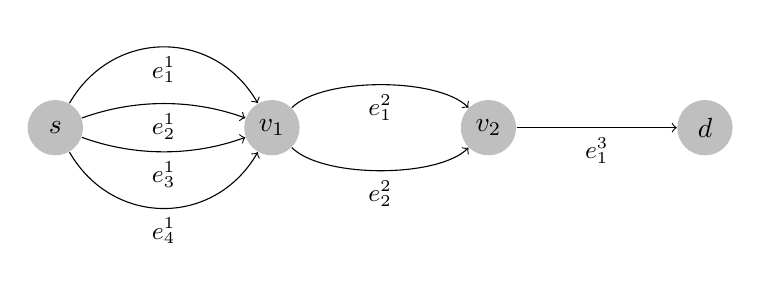
\begin{tikzpicture}[scale=0.55,auto,swap]
    \node[vertex](s1) at (0,0){$s$};
    \node[vertex](s2) at (5,0){$v_1$};
    \node[vertex](s3) at (10,0){$v_2$};
    \node[vertex](s4) at (15,0){$d$};

    \draw [edge] (s1) to[out=60,in=120, distance=2cm ] node[weight,below,black]{$e_1^1$} (s2);
    \draw [edge] (s1) to[out=20,in=160, distance=1.3cm ] node[weight,below,black]{$e_2^1$} (s2);
    \draw [edge] (s1) to[out=-20,in=200, distance=1.3cm ] node[weight,below,black]{$e_3^1$} (s2);
    \draw [edge] (s1) to[out=-60,in=240, distance=2cm ] node[weight,below,black]{$e_4^1$} (s2);
    
    \draw [edge] (s2) to[out=45,in=135, distance=1cm ] node[weight,below,black]{$e_1^2$} (s3);
    \draw [edge] (s2) to[out=-45,in=-135, distance=1cm ] node[weight,below,black]{$e_2^2$} (s3);

    \draw [edge] (s3) to[out=0,in=180, distance=1cm ] node[weight,below,black]{$e_1^3$} (s4);
 \end{tikzpicture}